\section{Experiments}
\label{sec:experiments}

The preceding sections specify the path measure, moves, OPES correction, and
symmetry context. We now apply the pipeline to a concrete protein--ligand
co-folding benchmark using the public Boltz-2 generator and OpenPathSampling
\citep{ops}. We first describe the system and Monte Carlo configuration, record
pseudocode aligned with the implementation, and then summarize unbiased TPS ensembles and TPS+OPES projections.

\subsection{System and Monte Carlo Configuration}

We study a $228$-residue two-chain heterodimer with protein--ligand co-folding
using the Boltz-2 multimer pipeline with multiple-sequence alignment (MSA)
information withheld. The padded atom tensor has $M = 1792$ atoms, the reverse
schedule has $L = 32$ steps, and the initial noise scale is
$\sigma_0 = 2560$~\AA{} (implementation convention matching the released
sampler). State volumes $A$ and $B$ are defined on the diffusion coordinate:
$A$ at high noise (disordered) and $B$ at low noise (structured), so every
accepted path is a complete denoising trajectory.

The path Markov chain uses the mixture from Section~\ref{sec:tps-foundations}:
forward shooting with probability $0.45$, backward shooting with probability
$0.45$, and global reshuffle with probability $0.10$, with a uniformly sampled
shooting index when applicable. Unbiased TPS runs for $N_{\mathrm{MC}} = 100$
Monte Carlo steps after initialization from a single forward pass. TPS+OPES
runs log every step to disk; the two-dimensional case study summarized below
used $N_{\mathrm{MC}} = 11\,590$ logged steps with $3\,184$ acceptances
($27.5\%$ acceptance rate).

\subsection{Algorithms}

\begin{figure}[t]
\hrule\vspace{2pt}
{\footnotesize\textbf{Algorithm 1.} TPS for a generic non-reversible generative model}
\vspace{1pt}\hrule\vspace{3pt}
{\footnotesize
\textbf{Require:} forward kernel $G$; noise priors $\pi_i$; state volumes $A,B$; initial reactive path $\mathcal{X}^{(0)}$ with $x_0\in A$, $x_L\in B$.
\begin{enumerate}\setlength{\itemsep}{0.15em}
  \item For each $k = 1,\ldots,N_{\mathrm{MC}}$:
  \begin{enumerate}\setlength{\itemsep}{0.1em}
    \item \textbf{Select} shooting index $i^* \sim \mathrm{Uniform}\{1,\ldots,L-1\}$.
    \item \textbf{Resample} $\xi_{i^*}^{\mathrm{new}} \sim \pi_{i^*}$ and $\xi_i^{\mathrm{new}}\sim\pi_i$ for all $i>i^*$.
    \item \textbf{Integrate} $x_{i+1}^{\mathrm{new}} = G(x_i^{\mathrm{new}}, \xi_i^{\mathrm{new}})$ for $i=i^*,\ldots,L-1$.
    \item \textbf{Reactivity:} if $x_L^{\mathrm{new}}\notin B$, reject and set $\mathcal{X}^{(k)}=\mathcal{X}^{(k-1)}$; continue to next $k$.
    \item \textbf{Log-ratio:} compute $\Delta$ via Eq.~\eqref{eq:delta} (forward) or Eq.~\eqref{eq:deltabwd-full} (backward).
    \item \textbf{Accept} $\mathcal{X}^{(k)}=\mathcal{X}^{\mathrm{new}}$ with probability $\min(1,e^{\Delta})$; otherwise keep $\mathcal{X}^{(k-1)}$.
  \end{enumerate}
\end{enumerate}}
\vspace{1pt}\hrule\vspace{2pt}
{\footnotesize\textit{Note.} The listing emphasizes \emph{forward shooting} (suffix resampled, prefix fixed, $\Delta = 0$ under Eq.~\eqref{eq:delta}). The production chain also uses \emph{backward shooting} (Hastings-corrected, Eq.~\eqref{eq:deltabwd-full}) and \emph{global reshuffle} (fresh $x_0 \sim \rho$ and all $\xi_i$).}
\vspace{1pt}
\label{alg:tps}
\end{figure}

\begin{figure}[t]
\hrule\vspace{2pt}
{\footnotesize\textbf{Algorithm 2.} TPS+OPES for a non-reversible generative model}
\vspace{1pt}\hrule\vspace{3pt}
{\footnotesize
\textbf{Require:} same $G$, $\pi_i$, $A,B$, $\mathcal{X}^{(0)}$ as Algorithm~1; CV map $\mathbf{s}(\cdot)$; bias factor $\gamma$; barrier height; kernel bandwidth $\sigma_{\mathrm{OPES}}$; deposition interval \texttt{pace}.
\begin{enumerate}\setlength{\itemsep}{0.15em}
  \item \textbf{Initialize} KDE state $\mathcal{K}_0\leftarrow\emptyset$ and $V_0(\mathbf{s})\leftarrow 0$.
  \item For each $k = 1,\ldots,N_{\mathrm{MC}}$:
  \begin{enumerate}\setlength{\itemsep}{0.1em}
    \item \textbf{Select and resample} as in Algorithm~1 (select $i^*$, resample suffix noise, integrate).
    \item \textbf{Reactivity:} if $x_L^{\mathrm{new}}\notin B$, reject; continue to next $k$.
    \item \textbf{Log-ratio:} compute $\Delta_{\mathrm{TPS}}$ from the unbiased TPS move.
    \item \textbf{CVs:} $\mathbf{s}^{\mathrm{n}} \leftarrow \mathbf{s}(x_L^{\mathrm{new}})$, $\mathbf{s}^{\mathrm{o}} \leftarrow \mathbf{s}(x_L^{(k-1)})$.
    \item \textbf{OPES bias:} $\Delta V \leftarrow V_{k-1}(\mathbf{s}^{\mathrm{n}}) - V_{k-1}(\mathbf{s}^{\mathrm{o}})$.
    \item \textbf{Accept} with probability $\min\bigl(1, \exp(\Delta_{\mathrm{TPS}} - \Delta V / k_BT)\bigr)$ (Eq.~\eqref{eq:tps-opes}); else keep the previous path.
    \item If $k \bmod \texttt{pace} = 0$, \textbf{deposit kernel} and update $V_k$ via Eqs.~\eqref{eq:opes-pn}--\eqref{eq:opes-vn}; else $V_k\leftarrow V_{k-1}$.
  \end{enumerate}
\end{enumerate}}
\vspace{1pt}\hrule\vspace{2pt}
{\footnotesize\textit{Note.} $\hat{\rho}_k$ is the compressed kernel-density estimate along CVs; see Section~\ref{sec:opes-theory} for the fixed-bias lemma and the adaptive-bias remark.}
\label{alg:tps-opes}
\end{figure}

\subsection{Unbiased TPS: Structural and Energetic Spread}

Across the unbiased TPS run ($100$ Monte Carlo steps), the shooting acceptance
rate is approximately $53\%$, consistent with a well-mixed shooting
distribution \citep{bolhuis2002}. All accepted paths remain reactive.

At every $10$ Monte Carlo steps we extract the terminal structure and record:
(i) C$\alpha$ root-mean-square deviation (RMSD) relative to the first accepted
structure, and (ii) total potential energy after OpenMM energy minimization.
The C$\alpha$ RMSD values span $0.48$--$0.69$~\AA{} with mean
$0.59 \pm 0.06$~\AA{}, indicating strong concentration of terminal structures
despite independent resampling of $(R_i,\tau_i,\varepsilon_i)$ along each path.
OpenMM energies fall in the range $-42{,}201$ to $-41{,}653$~kJ/mol (spread
$\approx 548$~kJ/mol), consistent with physically plausible minima for the
sampled conformations.

Figure~\ref{fig:distributions} summarizes these diagnostics when the plotting
assets are present in \texttt{docs/figs/}.

\begin{figure}[t]
  \centering
  \IfFileExists{fig_distributions_placeholder.pdf}{%
    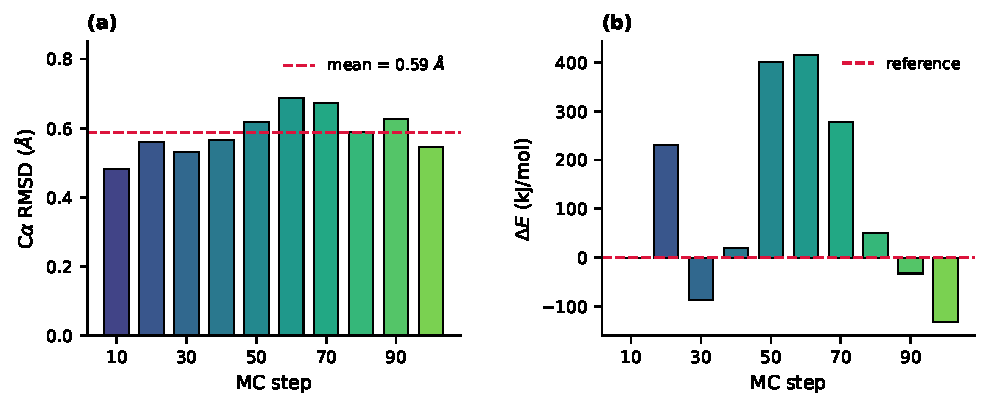
\includegraphics[width=0.72\linewidth]{fig_distributions_placeholder.pdf}%
  }{%
    \fbox{\begin{minipage}[c][0.28\textheight]{0.85\linewidth}\centering
    \vfill
    Place \texttt{fig\_distributions\_placeholder.pdf} in \texttt{docs/} to include the RMSD and energy panel.\\
    \vfill
    \end{minipage}}%
  }
  \caption{\textbf{Structural and energetic distributions of the unbiased TPS ensemble.}
  (a) C$\alpha$ RMSD of checkpoint structures relative to the first accepted structure
  (steps $10$--$100$). (b) OpenMM minimized energies (kJ/mol). Narrow RMSD spread
  indicates a sharply funneled denoising landscape for this input.}
  \label{fig:distributions}
\end{figure}

\subsection{Collective Variables for OPES and Diagnostics}

For the co-folding experiment, the two-dimensional OPES bias acts on
$\mathbf{s} = (s_1, s_2)$: $s_1$ is the ligand heavy-atom RMSD after Kabsch
alignment to a reference crystal pose (\AA), and $s_2$ is the ligand
center-of-mass to nearest binding-pocket C$\alpha$ distance (\AA) as
implemented in the repository. Small $s_1$ with moderate $s_2$ marks a
native-like basin; larger $s_1$ or shifts in $s_2$ track pose slippage and
pocket engagement changes. The published run used $\gamma = 10$, barrier
$5\,k_BT$, pace $1$, compression threshold $1.0$, ending with $1159$
depositions and $82$ compressed kernels.

The module \texttt{collective\_variables.py} logs additional geometry and
model-confidence scalars to \texttt{cv\_values.json} without feeding OPES:
contact order, steric clash counts, lDDT \citep{mariani2013lddt}, Ramachandran
outlier fractions, radius of gyration, Boltz mean pLDDT, and (for some
pipelines) OpenMM-relaxed C$\alpha$ RMSD. These are filters on plausibility and
memorization diagnostics, not terms in $P(\mathcal{X})$.

\subsection{TPS+OPES: Projected Landscape and Structures}

Figure~\ref{fig:opes2d} shows the three-panel summary (kernel mixture, a
reweighted free-energy proxy, and a visitation histogram) when
\texttt{docs/figs/opes\_tps\_ligand\_2d\_fes.png} is available. The dominant
peak near $(s_1, s_2) \approx (0.07~\mathrm{\AA},\,5.37~\mathrm{\AA})$ aligns
with the native-like basin; secondary structure near
$(0.70~\mathrm{\AA},\,5.55~\mathrm{\AA})$ and $(0.83~\mathrm{\AA},\,5.61~\mathrm{\AA})$
marks metastable pose basins at elevated ligand RMSD.

\begin{figure}[t]
  \centering
  \IfFileExists{figs/opes_tps_ligand_2d_fes.png}{%
    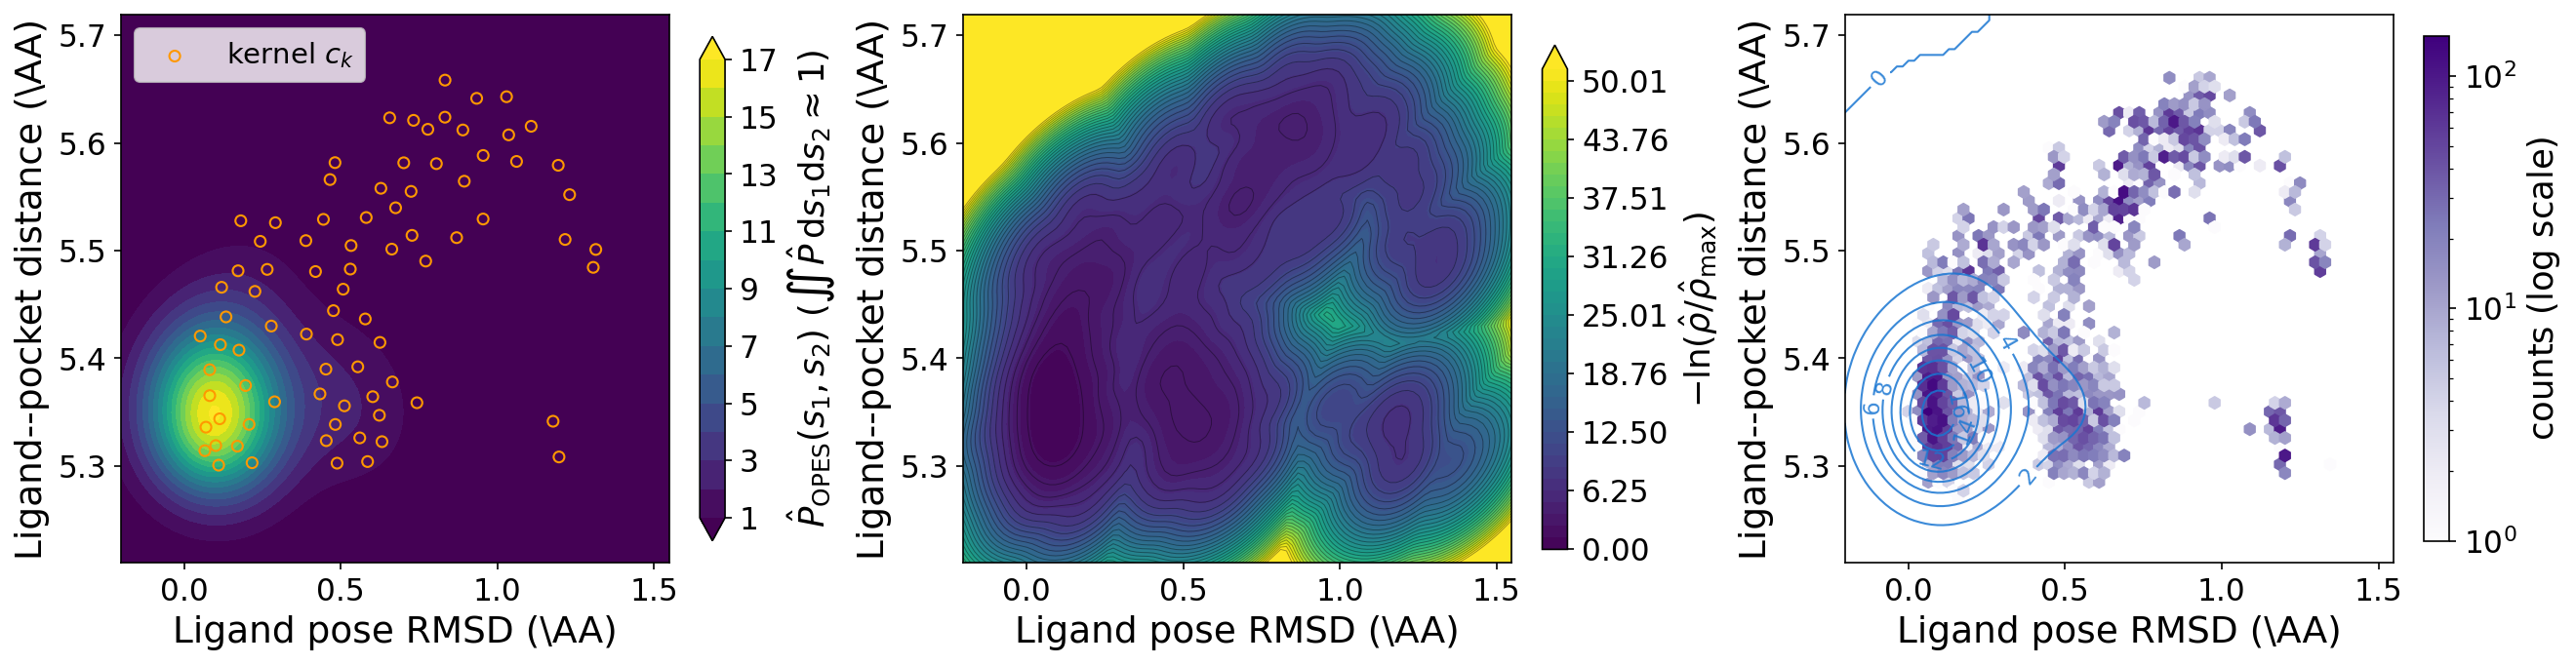
\includegraphics[width=0.92\linewidth]{figs/opes_tps_ligand_2d_fes.png}%
  }{%
    \fbox{\begin{minipage}[c][0.32\textheight]{0.9\linewidth}\centering
    \vfill
    Place \texttt{figs/opes\_tps\_ligand\_2d\_fes.png} under \texttt{docs/figs/} to include the triptych.
    \vfill
    \end{minipage}}%
  }
  \caption{\textbf{OPES--TPS two-dimensional summary in ligand pose space.}
  Kernel mixture, reweighted free-energy proxy, and visitation histogram with
  overlaid OPES contours (see repository scripts for regeneration).}
  \label{fig:opes2d}
\end{figure}

\begin{figure}[t]
  \centering
  \IfFileExists{figs/basin_structural_ensemble.png}{%
    \includegraphics[width=\linewidth]{figs/basin_structural_ensemble.png}%
  }{%
    \fbox{\begin{minipage}[c][0.35\textheight]{0.9\linewidth}\centering
    \vfill
    Place \texttt{figs/basin\_structural\_ensemble.png} under \texttt{docs/figs/} for basin-resolved structures.
    \vfill
    \end{minipage}}%
  }
  \caption{\textbf{Basin-resolved structural ensemble from TPS+OPES.}
  Representative terminal structures from metastable basins in the
  two-dimensional projection (cf.\ Figure~\ref{fig:opes2d}).}
  \label{fig:structures}
\end{figure}

Representative snapshots (Figure~\ref{fig:structures}, when available) show
native-like packing in the dominant basin and progressively displaced ligand
poses in higher-$s_1$ basins with modest increases in $s_2$, consistent with
geometrically distinct pocket engagement rather than pure rigid-body copies.

\subsection{Marginal Statistics and Run-Length Behavior}

Table~\ref{tab:cv-stats} reproduces the summary from
\texttt{scripts/summarize\_opes\_2d\_cv.py} on \texttt{opes\_tps\_out\_case1\_2d}.

\begin{table}[t]
\centering
\caption{Marginal CV statistics for the OPES--TPS two-dimensional run (case~1). ``All'' includes every logged step; ``Acc.'' conditions on accepted moves.}
\label{tab:cv-stats}
\begin{tabular}{lcccccc}
\toprule
 & \multicolumn{3}{c}{Ligand RMSD $s_1$ (\AA)} & \multicolumn{3}{c}{Pocket distance $s_2$ (\AA)} \\
\cmidrule(lr){2-4}\cmidrule(lr){5-7}
Subset & Mean $\pm$ SD & Median & $p_{95}$ & Mean $\pm$ SD & Median & $p_{95}$ \\
\midrule
All  & $0.49 \pm 0.35$ & $0.49$ & $1.19$ & $5.44 \pm 0.11$ & $5.40$ & $5.62$ \\
Acc. & $0.38 \pm 0.32$ & $0.26$ & $0.95$ & $5.41 \pm 0.10$ & $5.37$ & $5.61$ \\
\bottomrule
\end{tabular}
\end{table}

Among all logged steps, $48.9\%$ have $s_1 > 0.5$~\AA, $23.5\%$ exceed
$0.75$~\AA, $8.8\%$ exceed $1.0$~\AA, and $1.7\%$ exceed $1.25$~\AA.
Accepted paths show lower tail mass at the same thresholds ($36.6\%$,
$14.7\%$, $4.5\%$, $0.9\%$), reflecting the tension between OPES steering toward
high RMSD and the Metropolis filter that still favors paths with reasonable TPS
weights.

Run-length analysis on the stored chain shows that excursions with
$s_1 > 0.5$~\AA\ appear in sustained segments (mean length $39$ steps, maximum
$299$ over all logs), rather than isolated spikes. On accepted steps alone, the
mean run length above the same threshold is about $8$, still indicating
metastable dwell rather than single-point noise.

These empirical findings motivate the interpretation and limitations discussed
next.
